\documentclass[tikz,border=5pt]{standalone}
\usepackage{tikz}
\usetikzlibrary{patterns,arrows.meta}

\begin{document}
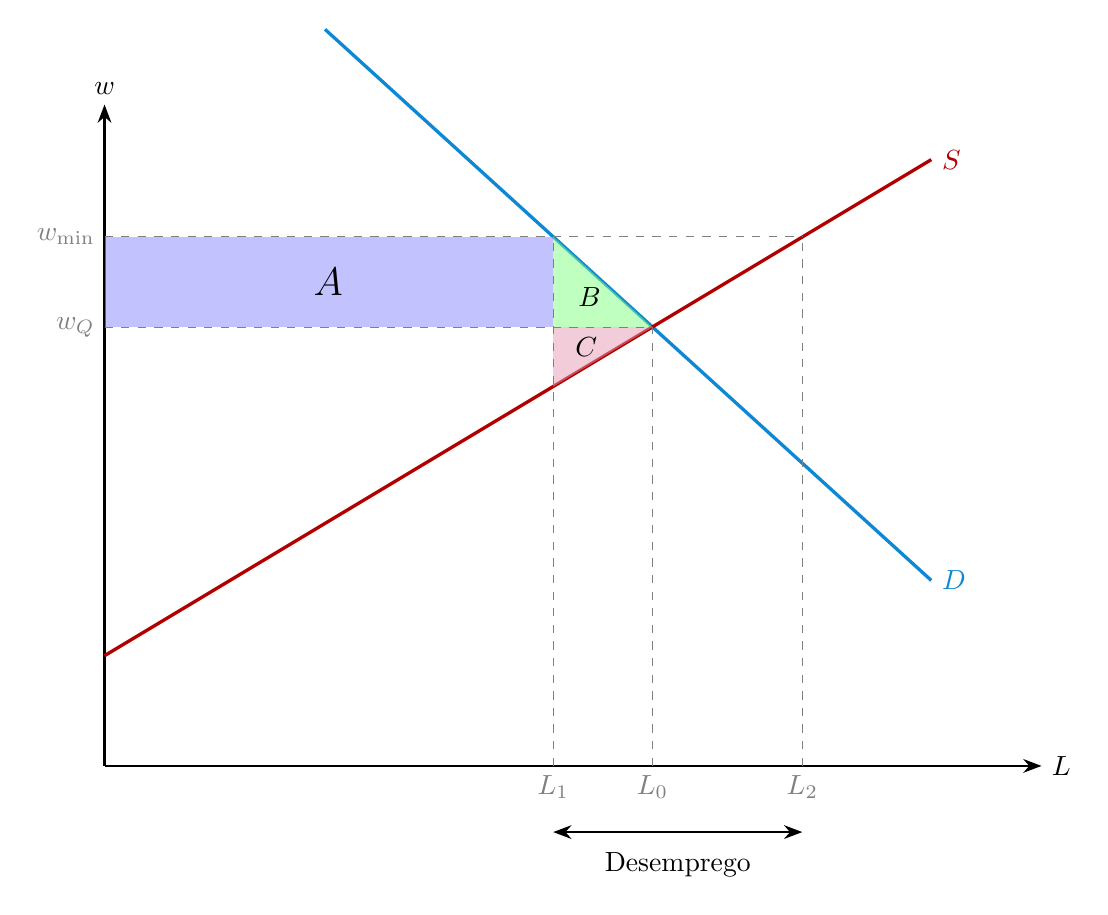
\begin{tikzpicture}[scale=1.4, >=Stealth]

  % Eixos
  \draw[thick,->] (0,0) -- (8.5,0) node[right] {$L$};
  \draw[thick,->] (0,0) -- (0,6) node[above] {$w$};

  % Curva de demanda (D) - azul, mesma da figura-9-07
  % y = 8.5 - 0.909*x
  \draw[cyan!70!blue, very thick, domain=2.0:7.5] plot (\x, {8.5 - 0.909*\x}) node[right] {$D$};

  % Curva de oferta (S) - vermelha, iniciando no eixo vertical, mesma da figura-9-07
  % y = 1.0 + 0.6*x
  \draw[red!70!black, very thick, domain=0:7.5] plot (\x, {1.0 + 0.6*\x}) node[right] {$S$};

  % Coordenadas dos pontos importantes
  % Ponto de equilíbrio (Q0) - interseção de S e D
  % 8.5 - 0.909*x = 1.0 + 0.6*x => x = 4.97, y = 3.98
  \coordinate (E) at (4.97, 3.98);
  
  % w_min (salário mínimo acima do equilíbrio)
  \def\Pmin{4.8}  % w_min
  \def\Peq{3.98}   % w_Q (equilíbrio)
  
  % L1: interseção de w_min com demanda D: 4.8 = 8.5 - 0.909*x => x = 4.07
  \coordinate (L1) at (4.07, 4.8);
  
  % L2: interseção de w_min com oferta S: 4.8 = 1.0 + 0.6*x => x = 6.33
  \coordinate (L2) at (6.33, 4.8);
  
  % Área A (retângulo - ganho dos trabalhadores empregados)
  \fill[blue!40, opacity=0.6] (0,\Peq) rectangle (4.07,\Pmin);
  
  % Área B (triângulo - perda de excedente do consumidor/empregador)
  \fill[green!50, opacity=0.5] (4.07,\Pmin) -- (4.97,\Peq) -- (4.07,\Peq) -- cycle;
  
  % Área C (triângulo - perda de excedente do produtor/trabalhador)
  % Oferta em x=4.07: y = 1.0 + 0.6*4.07 = 3.44
  \fill[purple!40, opacity=0.5] (4.07,3.44) -- (4.07,\Peq) -- (4.97,\Peq) -- cycle;

  % Linhas tracejadas horizontais
  \draw[dashed, gray] (0,\Pmin) node[left] {$w_{\min}$} -- (6.33,\Pmin);
  \draw[dashed, gray] (0,\Peq) node[left] {$w_Q$} -- (4.97,\Peq);

  % Linhas tracejadas verticais
  \draw[dashed, gray] (4.07,0) node[below] {$L_1$} -- (4.07,\Pmin);
  \draw[dashed, gray] (4.97,0) node[below] {$L_0$} -- (4.97,\Peq);
  \draw[dashed, gray] (6.33,0) node[below] {$L_2$} -- (6.33,\Pmin);

  % Rótulos das áreas
  \node at (2.03, 4.39) {\Large $A$};
  \node at (4.4, 4.25) {$B$};
  % Centro do triângulo C: ((4.07+4.07+4.97)/3, (3.44+3.98+3.98)/3) = (4.37, 3.80)
  \node at (4.37, 3.80) {$C$};

  % Seta de desemprego
  \draw[<->, thick] (4.07, -0.6) -- (6.33, -0.6);
  \node at (5.2, -0.9) {Desemprego};

\end{tikzpicture}
\end{document}
